\documentclass[aspectratio=169,12pt]{beamer}
\usepackage[T1]{fontenc}
\usepackage[utf8]{inputenc}
\usepackage[italian]{babel}
\usepackage{amsmath}
\usepackage{siunitx}
\usepackage{graphicx}
\usepackage{booktabs}
\usepackage{xcolor}
\usetheme{default}
\definecolor{deepblue}{RGB}{20,52,92}
\definecolor{accent}{RGB}{0,132,140}
\definecolor{warn}{RGB}{173,56,38}
\setbeamercolor{structure}{fg=deepblue}
\setbeamercolor{frametitle}{fg=white,bg=deepblue}
\setbeamercolor{title}{fg=deepblue}
\setbeamerfont{title}{size=\Huge,series=\bfseries}
\setbeamerfont{frametitle}{size=\large,series=\bfseries}
\setbeamerfont{normal text}{size=\large}
\setbeamertemplate{navigation symbols}{}
\setbeamertemplate{footline}{%
\leavevmode\hbox to \paperwidth{\hfill%
\insertframenumber/\inserttotalframenumber\hspace{1em}}%
\vskip0.5em}
\newcommand{\good}[1]{\textcolor{accent}{\textbf{#1}}}
\newcommand{\bad}[1]{\textcolor{warn}{\textbf{#1}}}
% Generated by build_m18_report_values.m. Do not edit.
\newcommand{\MOneMass}{1}
\newcommand{\MTwoMass}{0.8}
\newcommand{\LOneLength}{0.4}
\newcommand{\LTwoLength}{0.3}
\newcommand{\JmOne}{0.01}
\newcommand{\BmOne}{0.02}
\newcommand{\KOne}{50}
\newcommand{\KTwo}{40}
\newcommand{\GravityValue}{9.81}
\newcommand{\EquilibriumQOneDeg}{90}
\newcommand{\EquilibriumQTwoDeg}{0}
\newcommand{\OpenLoopMaxRealPole}{7.20943}
\newcommand{\ActuatorWn}{40}
\newcommand{\ActuatorZeta}{0.8}
\newcommand{\ActuatorDelayMs}{15}
\newcommand{\FullPlantOrder}{14}
\newcommand{\JmOneUncertaintyPct}{9}
\newcommand{\KOneUncertaintyPct}{7}
\newcommand{\KTwoUncertaintyPct}{7}
\newcommand{\MFourBlockCount}{5}
\newcommand{\SettlingTarget}{0.8}
\newcommand{\OvershootTarget}{10}
\newcommand{\ErrorTargetPct}{5}
\newcommand{\CrossTargetPct}{25}
\newcommand{\PerformanceBandwidth}{12}
\newcommand{\UScaleNm}{12}
\newcommand{\MControllerOrder}{14}
\newcommand{\MControllerWorstTs}{0.776}
\newcommand{\MSevenStatus}{PARTIAL}
\newcommand{\MSevenAdmissible}{0}
\newcommand{\MControllerRasMin}{60}
\newcommand{\MixsynGamma}{10.2071}
\newcommand{\HinfsynGamma}{10.2071}
\newcommand{\KhinfOrder}{18}
\newcommand{\AFiveGamma}{10.2477}
\newcommand{\AFiveRSLower}{0.875899}
\newcommand{\AFiveRSUpper}{0.882789}
\newcommand{\MusynObjective}{10.4032}
\newcommand{\BestDKIteration}{3}
\newcommand{\KmuOrder}{52}
\newcommand{\KmuNPStatus}{FAIL}
\newcommand{\KmuRSStatus}{PASS\_CERTIFIED}
\newcommand{\KmuRPStatus}{FAIL\_CERTIFIED}
\newcommand{\KmuRSLower}{1.25004}
\newcommand{\KmuRSUpper}{1.25257}
\newcommand{\KhinfRasMin}{52.8763}
\newcommand{\KmuRasMin}{60}
\newcommand{\MonteCarloSeed}{20260826}
\newcommand{\MonteCarloSamples}{40}
\newcommand{\MControllerStableSamples}{39}
\newcommand{\KhinfStableSamples}{40}
\newcommand{\KmuStableSamples}{40}
\newcommand{\MControllerSampleFivePole}{1.80447}
\newcommand{\MControllerTrackingPassPct}{30}
\newcommand{\KhinfTrackingPassPct}{0}
\newcommand{\KmuTrackingPassPct}{0}
\newcommand{\FinalRobustController}{Kmu}
\newcommand{\NominalReferenceController}{M6}
\newcommand{\HinfReferenceController}{Khinf}

\newcommand{\RevQs}{\num{0.08726646}}
\newcommand{\RevQds}{\num{1.047198}}
\newcommand{\RevDeltaScale}{\num{0.0125}}
\newcommand{\RevCareResidual}{\num{2.912849e-10}}
\newcommand{\RevRegulatorDecay}{\num{6.171691}}
\newcommand{\RevEstimatorDecay}{\num{9.31874}}
\newcommand{\RevSeparation}{\num{2.094409e-13}}
\newcommand{\RevRn}{\num{7.615435e-07}}
\newcommand{\RevCubicBound}{\num{18893}}
\newcommand{\RevHinfCrossover}{\num{13.83908}}
\newcommand{\RevTrajectoryFinalV}{\num{7.155528e-07}}
\newcommand{\RevTrajectoryIncrement}{\num{7.369284e-22}}

% Source: MATLAB export_hinf_final_results, summary.json
\newcommand{\FinalGamma}{0.0474606}
\newcommand{\FinalOrder}{22}
\newcommand{\FinalMuGamma}{0.63468}
\newcommand{\FinalMuOrder}{78}
\newcommand{\FinalMuObjective}{0.88381}
\newcommand{\FinalMinOrder}{2}
\newcommand{\FinalHRSLowerBound}{0.0181249}
\newcommand{\FinalHRSUpperBound}{0.0181617}
\newcommand{\FinalHRPLowerBound}{0.0172543}
\newcommand{\FinalHRPUpperBound}{0.0171945}
\newcommand{\FinalMuRSLowerBound}{1.7998}
\newcommand{\FinalMuRSUpperBound}{1.80442}
\newcommand{\FinalMuRPLowerBound}{1.67717}
\newcommand{\FinalMuRPUpperBound}{1.68066}

\title{Controllo robusto di un manipolatore planare 2-DoF con SEA}
\subtitle{Modellazione, sintesi e integrazione Simulink validata}
\author{Alessio de Dato \and Valerio Rebechi}
\date{Data di consegna: da completare}
\begin{document}

\begin{frame}[plain]\titlepage\end{frame}

\begin{frame}{La domanda di progetto richiede evidenze diverse}
\begin{itemize}
\item Modellare un manipolatore SEA non lineare e linearizzarlo.
\item Confrontare LQG, $H_\infty$ e $\mu$-synthesis.
\item Separare prestazione nominale, validazione non lineare, campionamento incerto e certificazione $\mu$.
\end{itemize}
\vfill
\good{Obiettivo finale: scegliere per ruolo, senza nascondere i risultati negativi.}
\end{frame}

\begin{frame}{L'elasticità separa link e rotori}
\[
M(q)\ddot q+C(q,\dot q)\dot q+G(q)=K_s(\theta-q)
\]
\[
J_m\ddot\theta+B_m\dot\theta=\tau-K_s(\theta-q)
\]
\begin{itemize}
\item Stato meccanico: $[q,\dot q,\theta,\dot\theta]$.
\item Equilibrio: $\bar q=[\EquilibriumQOneDeg^\circ,\EquilibriumQTwoDeg^\circ]^T$.
\item Il modello open-loop richiede controllo attivo.
\end{itemize}
\end{frame}

\begin{frame}{Attuatori e linearizzazione portano a 14 stati}
\begin{columns}[T]
\column{0.42\textwidth}
\begin{itemize}
\item $\omega_n=\ActuatorWn$ rad/s
\item $\zeta=\ActuatorZeta$
\item ritardo $\ActuatorDelayMs$ ms
\item Padé del primo ordine
\end{itemize}
\column{0.56\textwidth}
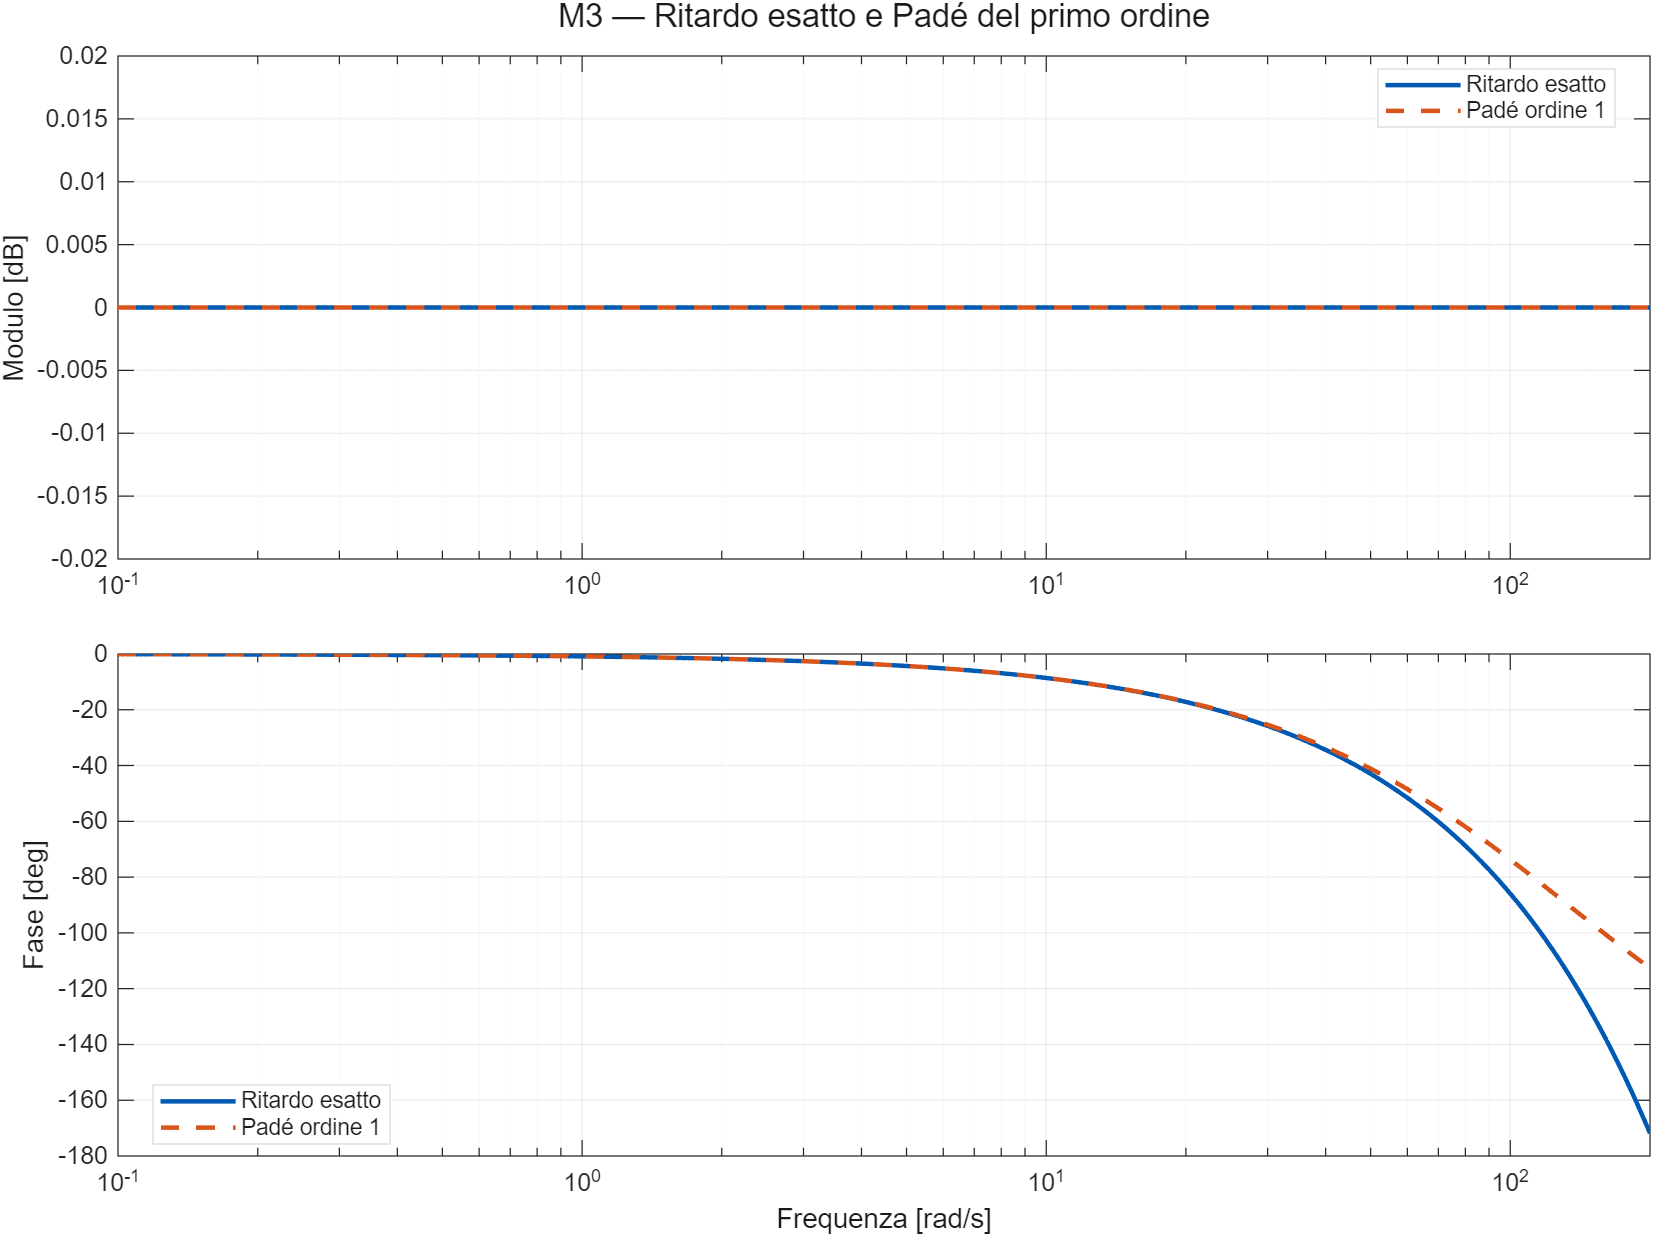
\includegraphics[width=\linewidth]{assets/m3_delay_pade_comparison.png}
\end{columns}
\end{frame}

\begin{frame}{M4 combina parametri reali e dinamica non modellata}
\begin{columns}[T]
\column{0.40\textwidth}
\begin{itemize}
\item $J_{m1}$: $\pm\JmOneUncertaintyPct\%$
\item $k_1,k_2$: $\pm\KOneUncertaintyPct\%$
\item due blocchi $\Delta_{act}$ indipendenti
\item range ingegneristici, non probabilità
\end{itemize}
\column{0.58\textwidth}
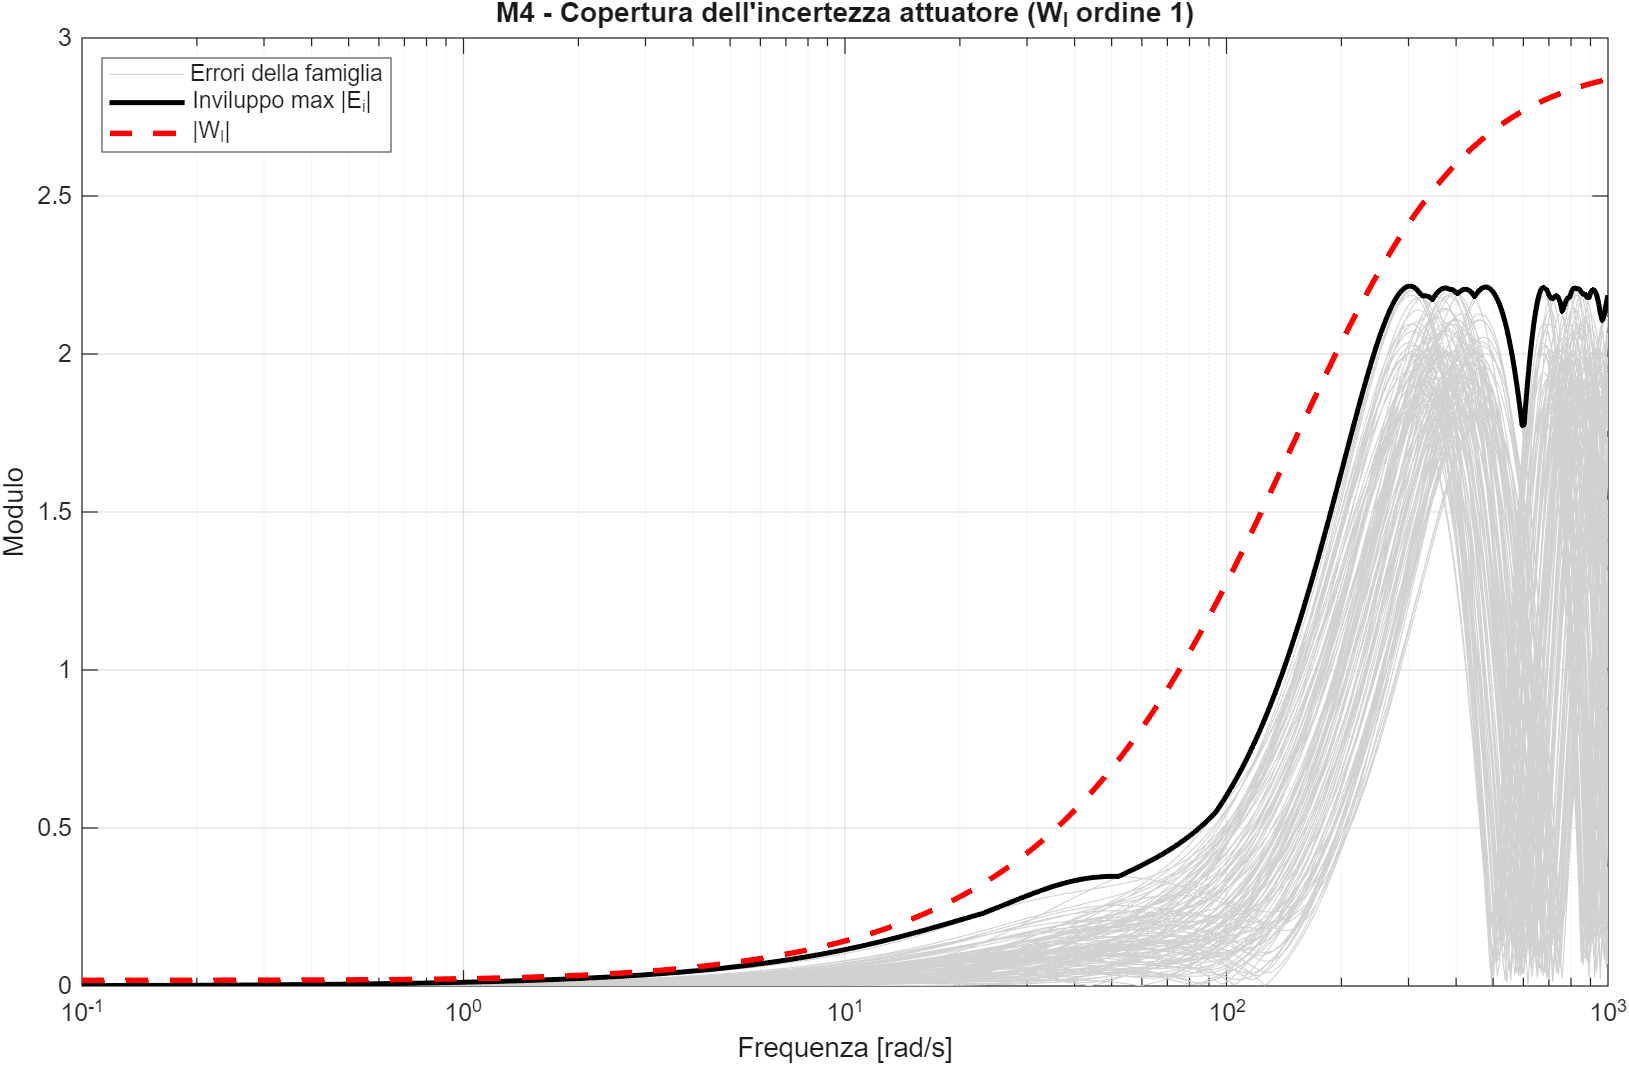
\includegraphics[width=\linewidth]{assets/m4_actuator_uncertainty_cover.png}
\end{columns}
\end{frame}

\begin{frame}{M5 fissa target e pesi prima del confronto}
\begin{columns}[T]
\column{0.40\textwidth}
\begin{itemize}
\item $T_s\leq\SettlingTarget$ s
\item overshoot $\leq\OvershootTarget\%$
\item errore $\leq\ErrorTargetPct\%$
\item cross-coupling $\leq\CrossTargetPct\%$ (diagnostico)
\end{itemize}
\bad{$u_{scale}=\UScaleNm$ N m non è una saturazione hardware.}
\column{0.58\textwidth}
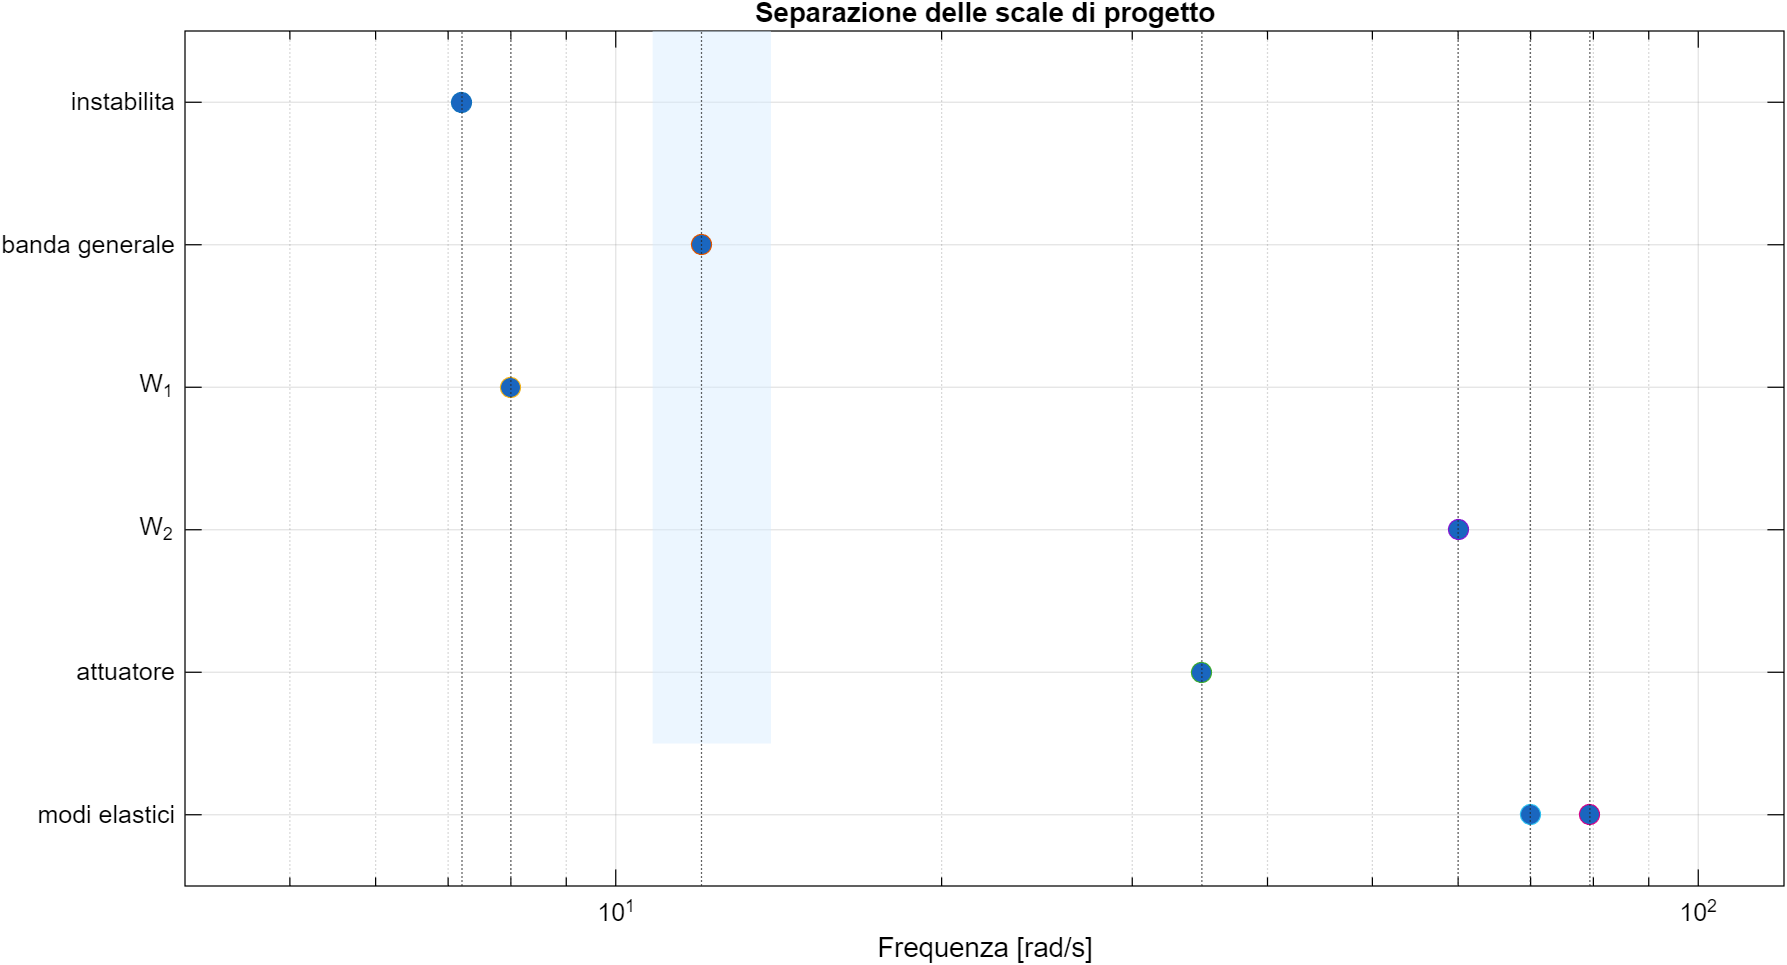
\includegraphics[width=\linewidth]{assets/m5_spec_frequency_map.png}
\end{columns}
\end{frame}

\begin{frame}{LQR: scale fisiche e pesi sono cose diverse}
\small
\[
v=[\Delta q;\Delta\dot q;\Delta\theta-\Delta q;\Delta\dot\theta]=Fx
\]
\[
\tilde v=S_x^{-1}Fx,\qquad
Q=F^TS_x^{-T}W_qS_x^{-1}F,\qquad R=r_u I_2
\]
\begin{columns}[T]
\column{0.48\textwidth}
Scale: $q_s=5^\circ$, $\dot q_s=12q_s$,
$\delta_s=0.5/40$ rad.

$r_u\in\{0.01,0.05,0.10\}$: pesi diretti.

\par\medskip
\bad{$q_s$ non è un peso di tuning.}
\column{0.48\textwidth}
Ricerca: \MLqrAdmissibleCount/\MLqrCandidateCount\ ammissibili.

$w_q=2,\ w_v=1,\ w_\delta=0.1,\ r_u=0.10$.

\par\medskip
$R=0.10I_2$; $Q$ non diagonale per $(\theta-q)^2$.
\end{columns}
\par\medskip
\[
Q,R\ \longrightarrow\ \mathrm{Riccati}\ \longrightarrow K
\ \longrightarrow\ \max\Re\lambda(A-BK)=-\RevRegulatorDecay
\]
\end{frame}

\begin{frame}{Kalman: ipotesi del progetto, non dati del docente}
\small
\[
\dot{\hat x}=A\hat x+Bu+L(y-C\hat x),\qquad y=[q;\theta]
\]
\begin{columns}[T]
\column{0.47\textwidth}
$\sigma_d=\sigma_u=0.1$ N m,
$\sigma_y=0.05^\circ$.

$Q_n=0.01I_4$,

$R_n=(0.05\pi/180)^2I_4$.

\par\medskip
Nessuna identificazione sperimentale.

\bad{Non confondere scala del rumore e sua varianza.}
\column{0.50\textwidth}
Sensibilità con lo stesso rumore applicato:
\begin{tabular}{rrr}\toprule
Fattore $\sigma_y$ & $\alpha_e/\alpha_c$ & RMS $\Delta u$ \\
\midrule
0.5 & 2.096 & 0.1499 \\
1 & 1.499 & 0.0819 \\
2 & 1.183 & 0.0428 \\
\bottomrule\end{tabular}
\par\scriptsize RMS in N m, passo 2 ms, 4 s, seed 20260826.\small

\par\medskip
Più fiducia nelle misure: stima più rapida, più rumore nel comando.
\end{columns}
\par\medskip
$u=-K\hat x+N_rr$: nel nominale lineare i poli LQG sono l'unione
dei poli di regolatore e stimatore.
\end{frame}

\begin{frame}{M6 è il riferimento di tracking nominale}
\begin{columns}[T]
\column{0.36\textwidth}
\begin{itemize}
\item LQG senza integratore
\item ricerca LQR: \MLqrAdmissibleCount/\MLqrCandidateCount\ casi ammissibili
\item selezionato \MLqrSelectedCandidate
\item ordine LQG \MControllerOrder
\item $T_s$ peggiore \MControllerWorstTs\ s
\end{itemize}
\column{0.62\textwidth}
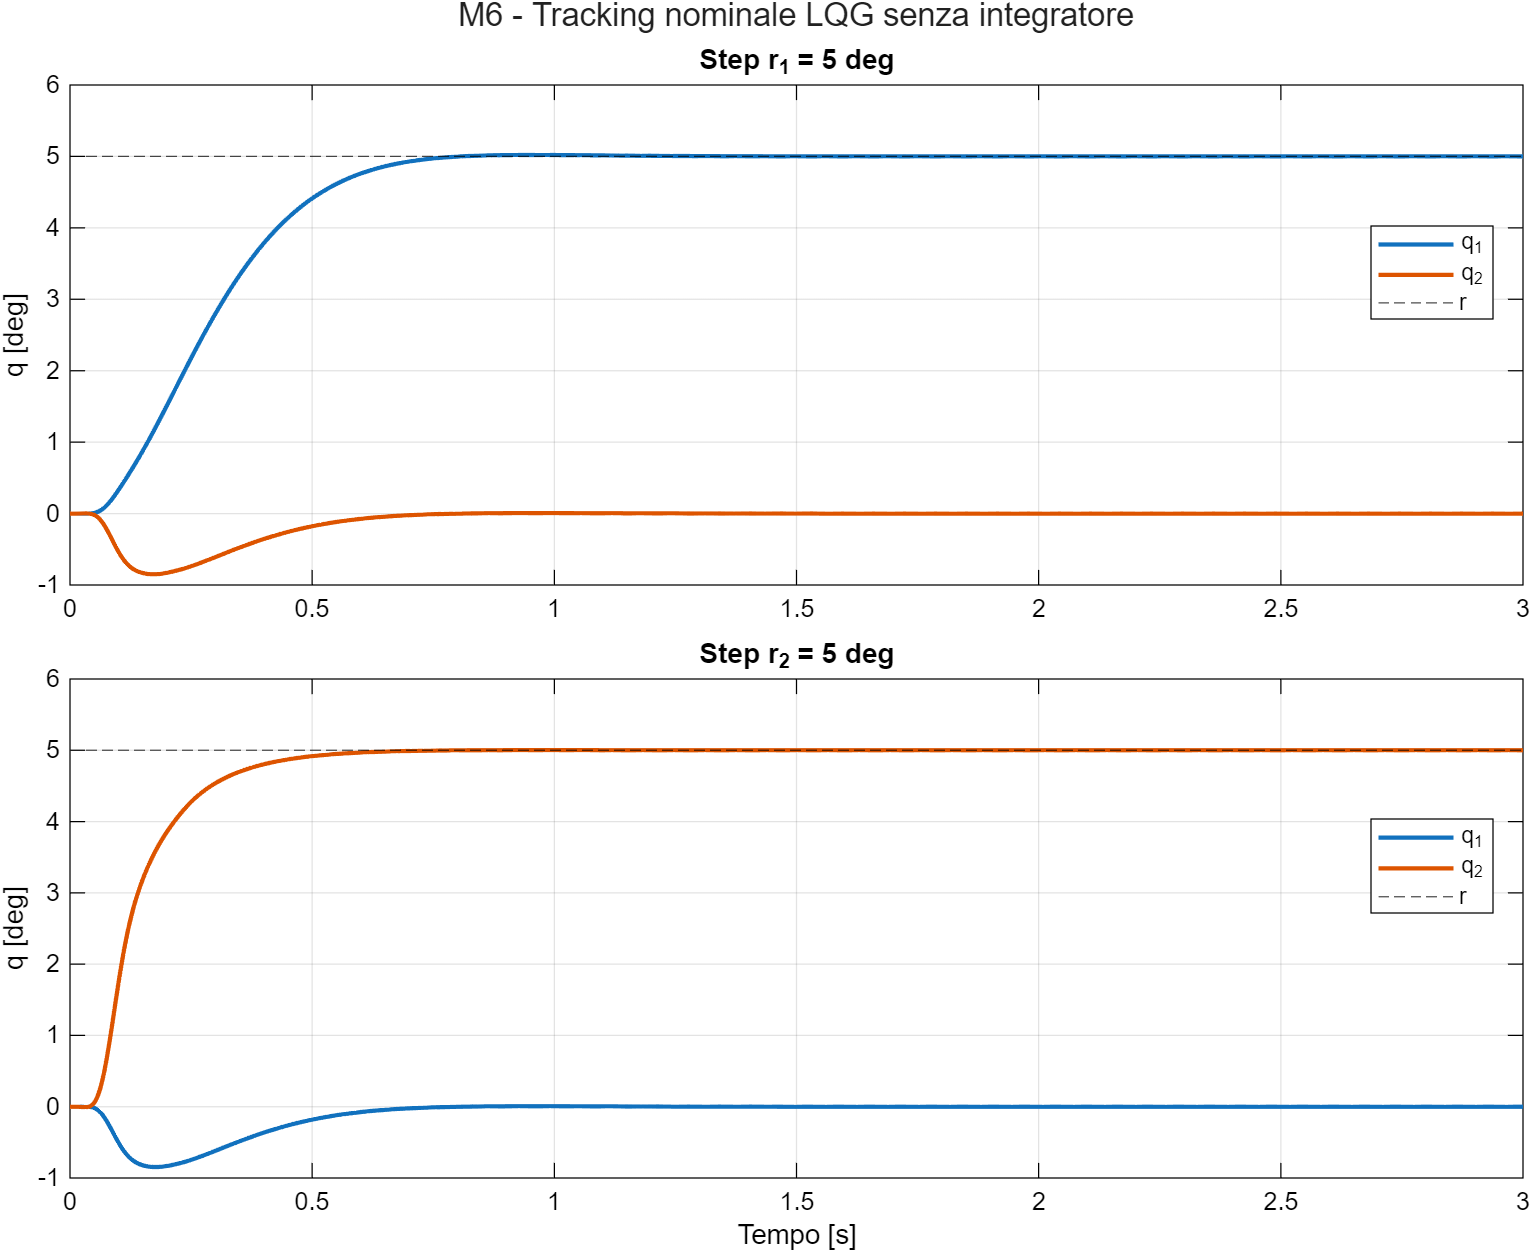
\includegraphics[width=\linewidth]{assets/m6_lqg_reference_tracking.png}
\end{columns}
\end{frame}

\begin{frame}{M7 chiude con un risultato negativo utile}
\begin{itemize}
\item LQRI con Kalman M6: 14 stati fisici, 14 stimati, 2 integratori.
\item Peso diretto $Q_i=\bar w_i I_2$, con $\bar w_i\in\{20,200,800\}$.
\item Verifiche conformi a tutti i requisiti: \MSevenAdmissible.
\item Nessuna verifica soddisfa insieme settling time e overshoot M5.
\end{itemize}
\vfill
\bad{Stato M7: \MSevenStatus. LQRI implementata, nessun candidato conforme.}
\end{frame}


\begin{frame}{Da una norma minore di uno a un vero progetto 2-DoF}
\begin{itemize}
\item La ricerca 1-DoF resta sovraelongata: $\gamma<1$ da solo non risolve il tracking.
\item Il controllore corrente riceve $[r;q]$ e produce due comandi.
\item $u=K_r r+K_yq$: i due rami condividono 22 stati interni.
\item Norma pesata nominale: \FinalGamma; nessun overshoot nominale.
\end{itemize}
\[z=\begin{bmatrix}W_e(q-M_or)\\W_u u\end{bmatrix},\quad
M_o(s)=\frac{16}{s^2+8s+16}I_2,\quad w=[r;d].\]
\bad{I target M5 restano invariati e non tutti soddisfatti.}
\end{frame}

\begin{frame}{H-infinity: tracking migliorato, robustezza insufficiente}
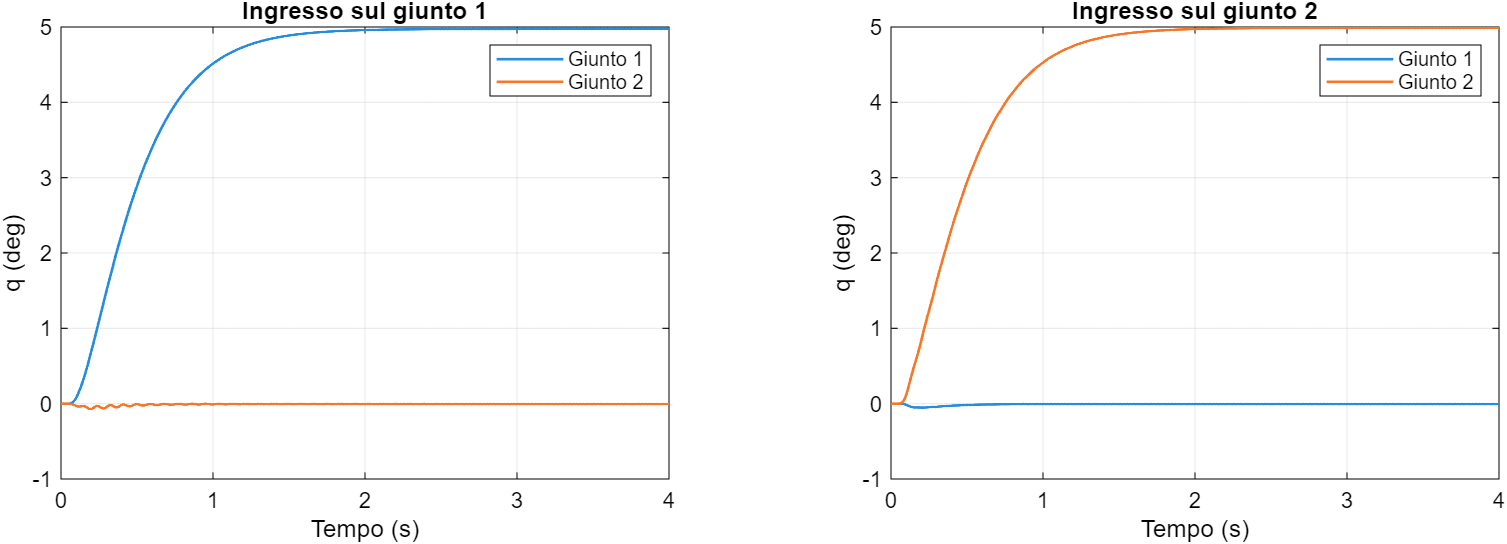
\includegraphics[width=\textwidth,height=.57\textheight,keepaspectratio]{../report/figures/hinf_final/tracking_2dof.png}
\begin{itemize}
\item $T_s\simeq1.46$ s: fallisce il target originale di 0.8 s.
\item NS/NP PASS; margine RS $[0.01812,0.01816]$: FAIL.
\item RP non accreditata: RS fallisce e l'intervallo numerico RP è invertito.
\end{itemize}
\end{frame}

\begin{frame}{Kmu è il candidato robusto del modello dichiarato}
\begin{itemize}
\item Stesso problema incerto 2-DoF, controllore completo di 78 stati.
\item Objective di sintesi \FinalMuObjective; norma nominale \FinalMuGamma.
\item Post-analisi: RS $[1.7998,1.8044]$, RP $[1.6772,1.6807]$.
\item NS, NP, RS e RP: PASS sul modello lineare incerto M4.
\end{itemize}
\vfill
\good{La post-analisi indipendente sostiene il ruolo robusto.}
\par\medskip
\bad{M5 resta FAIL: settling e offset del primo giunto.}
\end{frame}

\begin{frame}{Quaranta campioni comuni: esiti opposti}
\begin{columns}[T]
\column{.36\textwidth}
\begin{itemize}
\item H-infinity: 0/40 stabili.
\item Kmu: 40/40 stabili.
\item LQG storico: 37/40.
\end{itemize}
\par\medskip
Il campionamento è evidenza empirica; non definisce una probabilità fisica.
\column{.62\textwidth}
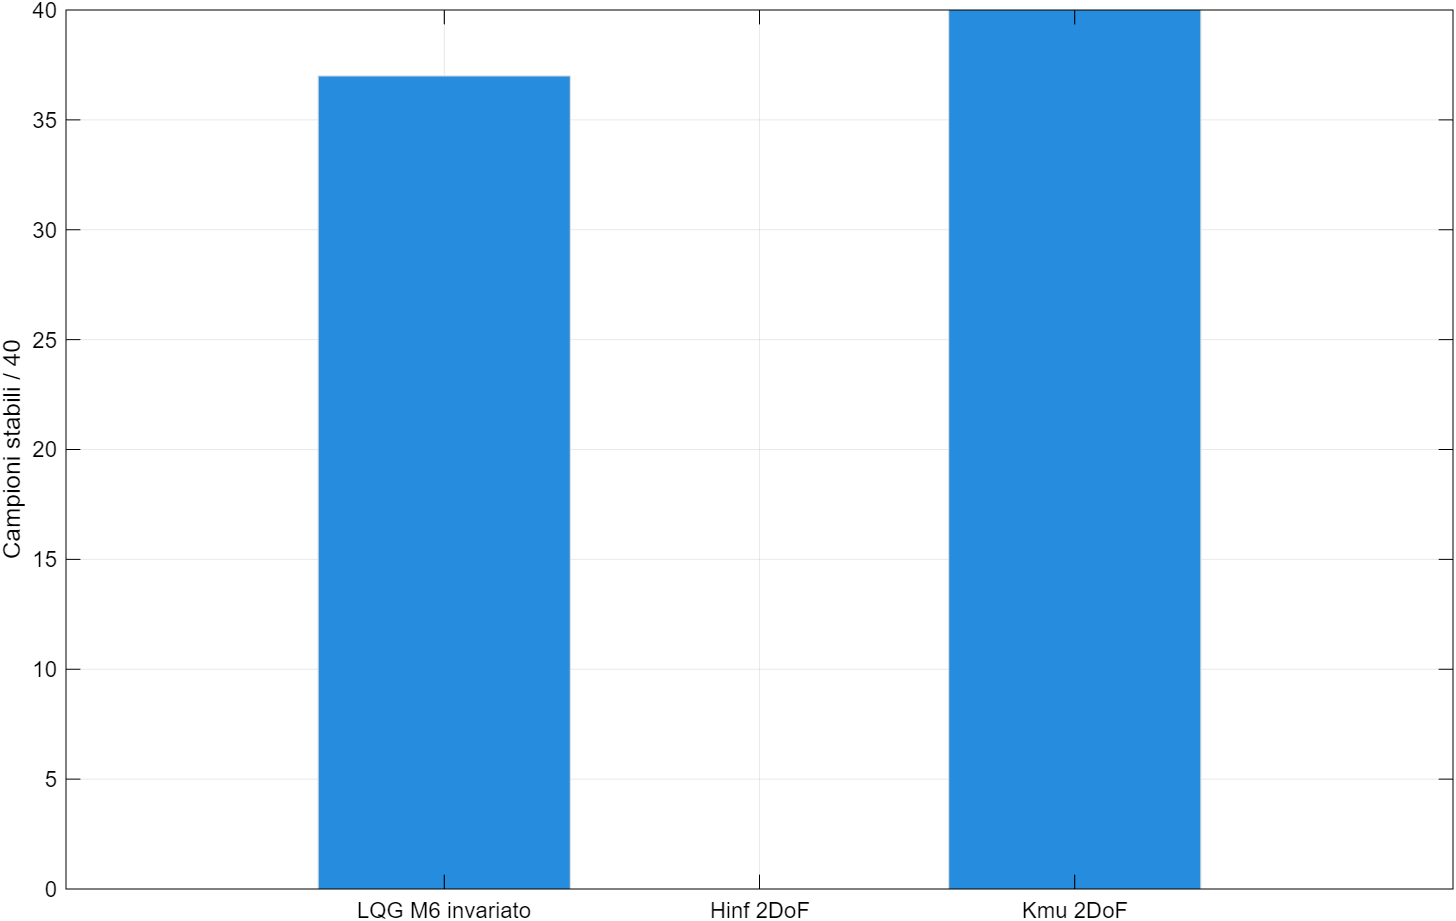
\includegraphics[width=\linewidth]{../report/figures/hinf_final/monte_carlo.png}
\end{columns}
\end{frame}

\begin{frame}{Rumore e regione di attrazione mostrano altri limiti}
\small
\begin{tabular}{lrr}\toprule
Campagna MATLAB corrente & H-infinity & Kmu\\\midrule
Picco comando, rumore 4 s [Nm] & 5685 & 8.12\\
RMS comando [Nm] & 118.2 & 1.934\\
Punti RAS convergenti & 27/285 & 57/57\\
Raggio minimo risolto [deg] & 0 & 60\\\bottomrule
\end{tabular}
\begin{itemize}
\item Raggio zero: limite della ricerca a risoluzione di un grado.
\item Kmu: frontiera limitata dal box di ricerca, non dall'hardware.
\item Nessuna saturazione identificata: picchi elevati restano dichiarati.
\end{itemize}
\end{frame}

\begin{frame}{Lyapunov: distinguere certificato e verifica campionata}
\[A_{cl}^{T}P+PA_{cl}=-I,\qquad V(z)=z^TPz.\]
\begin{itemize}
\item H-infinity, 36 stati: residuo 65.27; gate numerico FAIL.
\item Kmu, 92 stati: residuo 0.04493, inferiore alla soglia 0.1.
\item Kmu: livello interno analitico $\rho\simeq1.066\,10^{-12}$.
\item Livello 3.697 verificato su direzioni finite: non è un nuovo certificato.
\end{itemize}
\vfill
Le evidenze della PR 32 sono conservate; l'integrazione non le ricalcola.
\end{frame}

\begin{frame}{Simulink: due piante, la stessa architettura 8+6}
\small
\[x_{\rm mech}=[q;\dot q;\theta;\dot\theta]\in\mathbb R^8,
\qquad x_a\in\mathbb R^6.\]
\begin{itemize}
\item Quattro modelli non lineari conservati: coordinate assolute,
attuatori inizializzati all'equilibrio, feedback incrementale.
\item Un solo nuovo modello lineare comune, con i controllori congelati:
\end{itemize}
\[\dot x=A_{\rm full}x+B_{\rm full}u+B_{d,\rm full}d,
\quad y=C_{\rm full,Meas}x,\quad q=C_{\rm full,Q}x.\]
\begin{itemize}
\item LQG/LQRI ricevono $[r;y]$; H-infinity/Kmu ricevono $[r;q]$.
\item Ordini totali: 28, 30, 36, 92. Nessuna nuova sintesi o riduzione.
\item Originali di Valerio in legacy; parametri e guadagni dagli artifact MATLAB.
\end{itemize}
\end{frame}

\begin{frame}{Rumori, Kalman e integratore: segnali distinti}
\small
\[d_{\rm link}=d_{\rm ext}+w_d,\quad
u_{\rm abs}=\bar\tau+\delta u+\eta_u,\quad y_{\rm mis}=y_{\rm ideal}+v.\]
\[G_w=[B_d\ B],\quad Q_n=0.01I_4,\quad R_n=(0.05\pi/180)^2 I_4.\]
\[\dot{\hat x}=A\hat x+B\delta u+L(y_{\rm mis}-C\hat x).\]
\begin{columns}[T]
\column{.48\textwidth}
\textbf{LQG}\[\delta u=-K\hat x+N_rr.\]
Lo stato vero serve al confronto, non al feedback.
\column{.48\textwidth}
\textbf{LQRI}\[\delta u=-K_x\hat x-K_i\xi,\quad\dot\xi=r-q_{\rm mis}.\]
Due integratori, nessun $N_r$ aggiuntivo.
\end{columns}
\par\medskip
Quattro rumori di misura indipendenti, seed fissi, ZOH 0.002 s.
Prove a banda finita: non white noise continuo esatto.
\end{frame}

\begin{frame}{LQG e LQRI: disturbo costante e condizioni iniziali}
\small
{\centering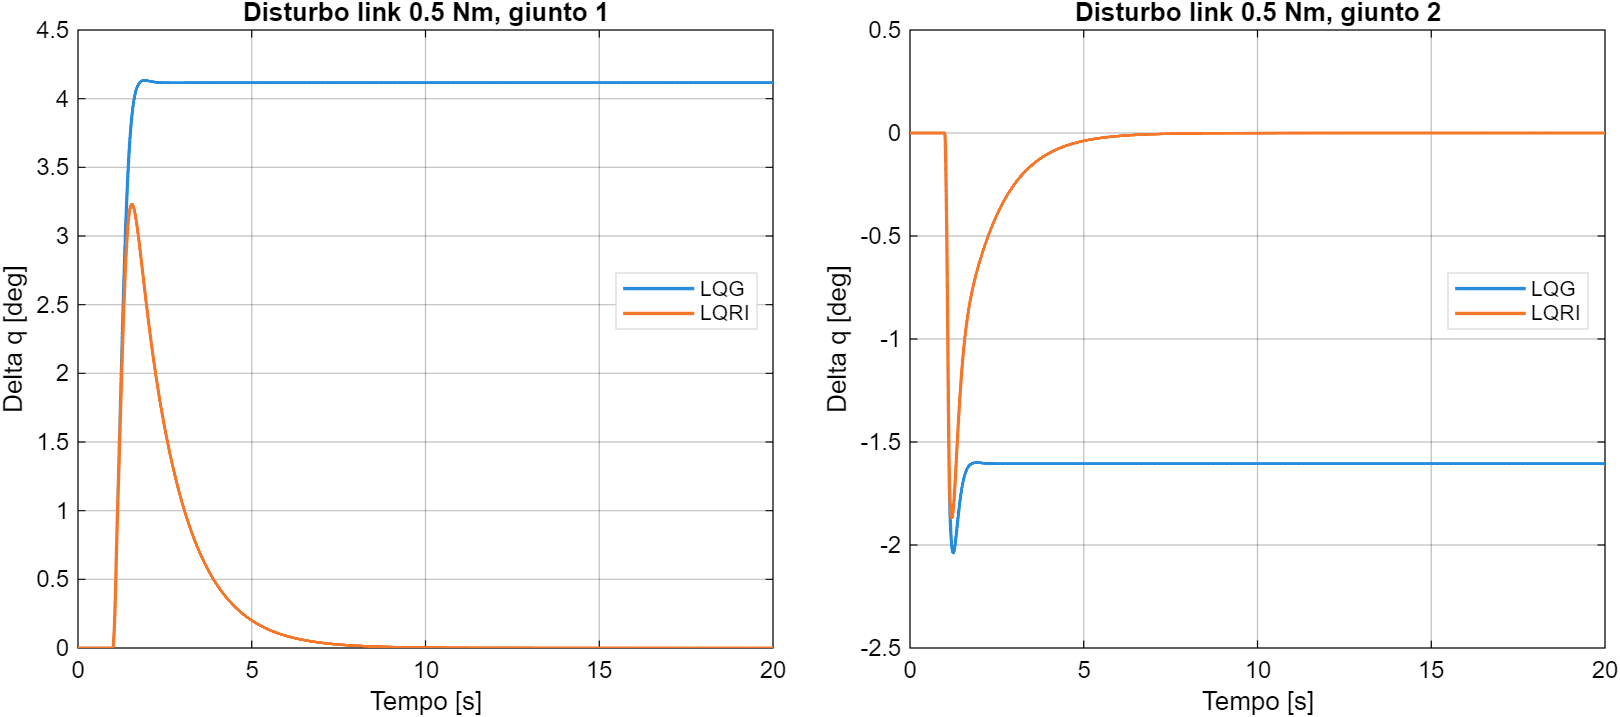
\includegraphics[width=\textwidth,height=.42\textheight,keepaspectratio]{../report/figures/simulink_integration/disturbance.png}\par}
\small
$d_1=0.5$ Nm da 1 s: a 20 s LQG mantiene offset;
LQRI lascia $\|e_q\|\simeq1.78\,10^{-8}$ rad.
\par\medskip
RAS nominale, stesso protocollo: \textbf{57/57 punti convergenti per entrambi},
box $\pm60^\circ$, 36 direzioni, precisione $1^\circ$, $\hat x_0=0$, $\xi_0=0$.
\par\medskip
\bad{Entrambe limitate dal box: nessuna RAS certificata o superiorità dimostrata.}
Picchi osservati: LQG 232.19 Nm, LQRI 240.96 Nm; M7 resta PARTIAL.
\end{frame}

\begin{frame}{Validazione completata, limiti di progetto conservati}
\small
\begin{tabular}{lrr}\toprule
Confronto, quattro controllori & max errore $q$ [rad] & max errore $u$ [Nm]\\\midrule
Simulink lineare / MATLAB lineare & 1.07e-08 & 1.79e-06\\
SL non lineare / lineare (piccolo segnale) & 9.80e-10 & 1.49e-07\\\bottomrule
\end{tabular}
\par\medskip
\good{32/32 nuovi controlli; 15/15 nuovi test e 7/7 originari PASS.}
Le evidenze originarie 67/67 restano invariate.
\begin{itemize}
\item LQG: riferimento nominale. LQRI: reiezione del disturbo costante.
\item Kmu: RS/RP PASS sul modello M4; H-infinity: RS FAIL.
\item M5 resta FAIL per i due robusti. Nessuna nuova garanzia hardware.
\item Simulato su R2025b; saturazioni, code generation e replay R2026a non verificati.
\end{itemize}
\end{frame}
\end{document}
